%----------------------------------------------------------------------------
\chapter{Irodalomkutatás}
\label{sec:Search}
%----------------------------------------------------------------------------

\section{Felhasznált technológiák}
\label{sec:Technologies}

Ebben a fejezetben bemutatom az általam használt technológiákat amiket használtam és segítettek ennek a dolgozatnak a megírásában és elkészítésében.

\subsection{Jetpack Compose}
\label{sec:Compose}

A Jetpack Compose a korábbi Android fejlesztési módszer mellett hozott létre egy alternatív megoldást.
Kezedtebn nem lehetett tudni, hogy a fejlesztők hogyan fognak reagálni az új irányra.
Korábban a Java nyelv mellett megjelent a Kotlin nyelv is, ami később szinte teljesen leváltotta az elődjét.
Ebből arra lehetett következtetni, hogy egy új és modernebb megoldás meg tudja állni a helyét az XML View megoldást ellenében.
Jelenleg mind a két megoldás támogatott, de a fejlsztések iránya egyértelműen a Compose felé húz.

"A Jetpack Compose egy új, deklaratív UI toolkit, amit a Google hozott létre kifejezetten natív Android alkalmazások fejlesztéséhez."\cite{GettingStartedWithJetpackCompose}
A deklaratív nyelvekhez hasonlóan, azt kellmegadnunk, hogy mit szeretnénk látni és nem azt leírni, hogy ez hogyan történjen meg.
Nekünk elegendő azt leírni, hogy a gomb hogyan nézzen ki és hol legyen és megadni egy lambda paraméternek, hogy a megnyomása soránmi történjen.
Mivel ez egy UI toolkit, ezért az összes vezerlő és szerkezeti elem hasonlóan néz ki, hasonlóan lehet használni így a fejlesztői és a felhasználói élmény is egységes és megszokott minőségű lesz minden alkalommal.
A Google ezt a Material design segítségével hozta létre, illetve annak újabb változataival. Erről részletesebben itt találhatók információk: \url{https://m3.material.io/}.

Az alábbiakban egy a Google által írt rövid kódrészleten (\ref{lst:compose}.~kódrészlet) bemutatom a legfontosabb részeit a Compose alapjainak.\cite{BasicCodelab}
Az első lépése az alaklamzás elkészítésének az a Composable függvény megírása.
Minden a UI-t megjelenítő függvény a @Composable annotációt viseli.
Innentől kezdve hagyományos Kotlin függvényként viselkedik, megadahatunk tetszőleges paramétereket (name, modifier) és alapértelmezett értékeket is.
Egy Composable függvényből tetszőleges másik Composable függvény meghívható megfelelőláthatóság esetén.
Ilyen például a Text() is ami a Material könyvtárnak egyik tagja és egyszerű szöveget jelenít meg.

A UI megírása után ezt a megfelelő helyen meg is kell jelenítenünk, erre az alkalmazás belépési pontja után van lehetőségünk.
Android esetén ez az activity onCreate függvénye.
A setContent vár egy lambda függvényt, aminek viselnie kell a @Composable annotációt, használhatjuk hozzá a Kotlin trailing lambda megoldását, aholis, ha az utolsó paramétere a függvénynek egy lambda, akkor a többi paraméter megadása után {} között megadhatjuk afüggvény törzsét.
A BasicsCodelabTheme is egy Composable függvény amiben az alap beállítások után meghívhatjuk a saját Greeting függvényünket.
A UI felépítse innentől kezdve már egyszerű.
A Composable függvények megírása után egymásból meghívva azokat előáll az alkalmazás.

\begin{lstlisting}[caption={Példa a Compose használatára.}, label={lst:compose}, language=Kotlin]
    @Composable
    fun Greeting(name: String, modifier: Modifier = Modifier) {
        Text(
            text = "Hello $name!",
            modifier = modifier
        )
    }

    class MainActivity : AppCompatActivity() {
        override fun onCreate(savedInstanceState: Bundle?) {
            super.onCreate(savedInstanceState)
            setContent {
                BasicsCodelabTheme {
                    // A surface container using the 'background' color from the theme
                    Surface(
                    modifier = Modifier.fillMaxSize(),
                    color = MaterialTheme.colorScheme.background
                    ) {
                        Greeting("Android")
                    }
                }
            }
        }
    }

    // Jetpack Compose forráskód
    public fun ComponentActivity.setContent(
        parent: CompositionContext? = null,
        content: @Composable () -> Unit
    )
\end{lstlisting}

A következőkben bemutatom a UI toolkit fontosabb általam használt részeit.
Kitérek arra, hogy mire jó, miért ezt használtam és hogyan lehet őket hatékonyan felhasználni a legújabb Compose Multiplatform verziókban.

\subsubsection{State és StateFlow}
\label{sec:State}

A State és a StateFlow hasnló problémára ad megoldást.
A State alapvetően Compose sepcifikus megoldás, ha változik az értéke akkor a lefut a recomposoition.
Ezzel szemben a StateFlow a Kotlin nyelvben általánosan használt eszköz és sokkal bővebb felhasználással rendelkezik, mint az egyszerű State.
Az egyszerű Stateet általában egy Composable függvényen belül használják, míg a a StateFlowt ViewModelekben.
Ennek ellénére mind a két megoldás tökéletesen alkalmazható, jelenleg már Compose Multiplatform alkalmazásokban is.
Mivel ViewModelben használva az adatok nem besznek el a képernyő elforgatása során ezért egyszerűbb műveletekre és adaokra nincs lényegi különbség a működésben. 

"A StateFlow előnyei:"\cite{StateVsStateFlow}
\begin{itemize}
    \item \emph{"Flow operátorok:} A StateFlow támogat olyan operátorokat, mint a map, filter, és combine, lehetővé téve az adatok rugalmas feldolgozását és összetett adatfolyamok létrehozását."
    \item \emph{"Folyamat-megszakadás kezelése:} A SavedStateHandle-lel kombinálva biztosítja az UI állapot megőrzését, még a képernyő elforgatása vagy újraindítás esetén is."
    \item \emph{"ViewModel újrafelhasználhatóság:} A StateFlow lehetővé teszi a ViewModel függetlenítését a UI-rétegtől, ami elősegíti a moduláris, tesztelhető és újrafelhasználható architektúrát."
\end{itemize}

A lenti kódban (\ref{lst:state}.~kódrészlet) láthatunk példát mind az egyszerű State használatára, ebben az esetben a Screen állapotát tárolom el Statekben.
A megjelnített adatok itt a StateFlow logikáját követik. 
Létezik egy privát MutableStateFlow amin történnek a változások például, ha adat érkezik.
Van egy másik azonos nevű érték is ami ugyan annak a StateFlownak egy immutábilis változata, ehhez fér hozzá a UI, így onnan nem érkezhet változás közvetlenül a StateFlowba.
Amennyiben erre szükség van, a viewmodel biztosíthat erre vonatkozóan függvényeket és beállíthatja a privát MutableStateFlow értékét.

\begin{lstlisting}[caption={Példa a State és StateFlow használatára.}, label={lst:state}, language=Kotlin]
class TopicListViewModel: ViewModel() {
    var topicListScreenUiState: TopicListScreenUiState by mutableStateOf(TopicListScreenUiState.Loading)
    private val _topicListUiState = MutableStateFlow(TopicListUiState())
    val topicListUiState: StateFlow<TopicListUiState> = _topicListUiState
...
    fun getAllTopicList(){
        topicListScreenUiState = TopicListScreenUiState.Loading // State Változás
        viewModelScope.launch {
            topicListScreenUiState = try{    // State Változás
                val result = ApiService.getAllTopicNames()
                _topicListUiState.value = TopicListUiState(     //StateFlow Változás
                    topicList = result.map { nameDto ->
                        TopicRowUiState(
                            topic = nameDto.name,
                            id = nameDto.uuid
                        )
                    }
                )
                TopicListScreenUiState.Success(result) // State Változás
            } catch (e: IOException) {
                TopicListScreenUiState.Error.errorMessage = e.toString()// "Network error"
                TopicListScreenUiState.Error // State Változás
            }
        }
    }
}
\end{lstlisting}

\subsubsection{ViewModel}
\label{sec:ViewModel}

Az Android ViewModel már használható Kotlin- és Compose Multiplatform környezetekben is\cite{ViewModelKMP}, így természetesen ezt a jól bevált megoldást választottam.
Egy rövid összefoglalót szeretnék adni a hivatalos dokumentáció alapján a képességeiről:\cite{ViewModelAndroid}

A ViewModel az Android Jetpack része, és az UI állapotának megőrzésére szolgál konfigurációs változások során, például képernyőforgatáskor. \refstruc{fig:ViewModel} Fő előnyei közé tartozik az állapot tartósítása és az üzleti logika elérése a UI-rétegben. A ViewModel segít elválasztani az adatkezelést a UI-rétegtől, ehhez a ViewModelben felhasználható a Kotlin coroutine ami egyfajta aszinkron működést tesz lehetővé, és kompatibilis olyan Jetpack könyvtárakkal, mint a Hilt, Compose, és a Navigation. Best practice szerint kerülni kell az életciklushoz kötött objektumok tárolását benne, hogy elkerüljük a memóriaszivárgást. 

Mint minden MVM és MVVM architektúrában az adatok elérése, átalakítása a UI számára, tartós tárolása a ViewModel feladata.
Több megközelítés is lehetséges: minden képernyő kapjon egy saját ViewModelt; egy ViewModel tudjon többet és legyen újra felhasznáva több képernyőn.
Én az első megoldást választottam, így könnyebb kezeleni a különböző képrenyők állaptait és egyszerűbb átlátni egy-egy egységet.

\begin{figure}[!ht]
    \centering
    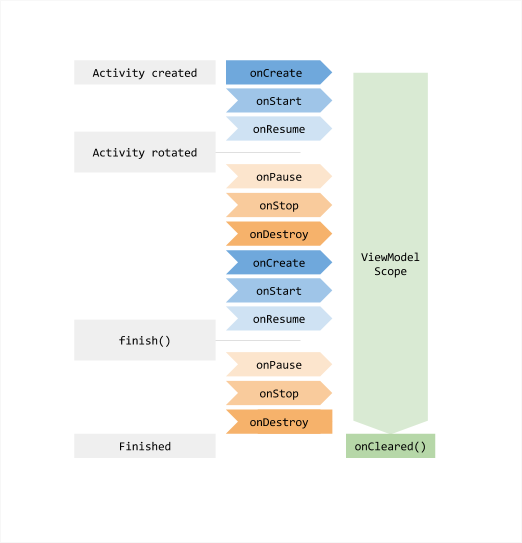
\includegraphics[width=150mm, keepaspectratio]{figures/viewmodel-lifecycle.png}
    \caption{A ViewModel álltalánosságban véve hosszabb életű, mint egy View. Ez különsöen igaz Android környezetben, ahol számolni kell a képernyő elforgatással és az alaklmazás háttérbe kerülésével. A tartósan tárolnikívánt adatokat ezért mindig ViewModel kell tárolni. \cite{ViewModelAndroid}}
    \label{fig:ViewModel}
\end{figure}

\subsubsection{Navigation and routing}
\label{sec:Navigation}

Az Androidban már jól műküdő navigációrt felelős könyvtárak már használhatóak a Kotlin Multiplatform fejlesztéséhez \cite{NavigationKMP}.
Ennk mindösszesen pár egyszerű lépése van, így könnyű használni és rugalamsan működik minden környezettel.
Mindezt kódvab is bemutatom. (\ref{lst:nav}.~kódrészlet)
A következők a szükséges lépések: \cite{NavigationKMP}.
\begin{enumerate}
    \item "Sorold fel a navigációs gráfban szereplő útvonalakat, mindegyik egyedi string határozza meg az útvonalat."
    \item "Hozz létre egy NavHostController példányt a navigáció kezeléséhez"
    \item "Adj hozzá egy NavHost komponenst az alkalmazásodhoz:"
        \begin{itemize}
            \item "Válaszd ki a kezdő útvonalat a korábban definiált útvonalak közül."
            \item "Hozd létre a navigációs gráfot közvetlenül a NavHost részeként vagy programozottan a NavController.createGraph() függvénnyel."
        \end{itemize}
\end{enumerate}

\begin{lstlisting}[caption={Példa a Navigation használatára.}, label={lst:nav}, language=Kotlin]

//Első lépés: útvonalak létrehozása
//Érdemes sealed classt használni és data objectként létrehozni a routeokat
sealed class ExamDestination(val route: String) {
    //Lehet egyszerű
    data object LoginScreenDestination : ExamDestination("LoginScreen")

    //Vagy paraméterekkel és adatokkal ellátott
    data object TopicDetailsDestination : ExamDestination("TopicDetails") {
        const val topicIdArg = "0"
        val routeWithArgs = "$route/{$topicIdArg}"
    }
}

//Második lépés: NavController létrehozása
fun NavigationComponent() {
    MaterialTheme {
        val navController = rememberNavController() //Itt történik
        Scaffold() { innerPadding ->
            ExamNavHost(    //Paraméternek egy Composable függvényt vár, ezen belül is egy NavHost függvényt
                navController = navController,
                modifier = Modifier.padding(innerPadding)
            )
        }
    }
}

//Harmadik lépés: NavHost komponens hozzáadása
actual fun ExamNavHost(
    navController: NavHostController,
    modifier: Modifier
) {
    NavHost(
        navController = navController,  //NavController hozzárendelése
        startDestination = ExamDestination.MainScreenDestination.route, //Kezdő útvonal beállítása
        modifier = modifier
    ) {
        //Navigácós gráf egy elemének létrehozása
        composable(
            route = ExamDestination.TopicListDestination.route,
        ) {
            TopicListScreen(
                addNewTopic = { navController.navigate(ExamDestination.NewTopicDestination.route) },
                navigateToTopicDetails = { topicId ->
                    navController.navigate("${ExamDestination.TopicDetailsDestination.route}/${topicId}")
                },
                navigateBack = { navController.popBackStack() }
            )
        }
    }
}
\end{lstlisting}

\section{Ktor}
\label{sec:Ktor}

A Ktor egy Kotlin HTTP kommunikációt megvalósító könyvtár\cite{Ktor}. Alkalmas mind szerver oladli kód írásárá, a REST API-om is ezt használja és kliens oladli kód megvalósítsára is.
A használata nagyon egyszerű, és testreszabható.
Én egy Kotlin objectet használtam, ami magában foglalja az ApiServicet.
Létre kellett hozni egy http klienst és beállítani a base url-t, illetve a content typenak a JSON üzenet formátumot.
Ezt követően a végpont hívásokat kellett már csak létrehozni.


\begin{lstlisting}[caption={Példa a Ktor használatára.}, label={lst:ktor}, language=Kotlin]
object ApiService {
    private var authToken: String? = null  // Mutable token that can be updated at runtime

    private val httpClient = HttpClient() {
        install(ContentNegotiation) {   // content type beállítása
            json(Json {
                ignoreUnknownKeys = true
                prettyPrint = true
            })
        }

        defaultRequest {    // Base url beálítása
            url("http://mlaci.sch.bme.hu:46258")  // Set the base URL   152.66.182.70:46258   192.168.1.17:46258
            authToken?.let { token ->
                header(HttpHeaders.Authorization, "Bearer $token")  // Add the Bearer token if it's not null
            }
        }
    }
    suspend fun getAllPoints(): List<PointDto> = httpClient.get("/point").body()    //végpontok
}
\end{lstlisting}

\section{KotlinX Serilizáció}
\label{sec:KotlinX}

A serilizáció a JSON formátum konvertálása miatt van szükség. Az alábbiakban a hivatalos dokumentációból olvasható egy részlet ami jól összefoglalja a használatát.
Ez a technológia is használható Kotlin Multiplatform területen.

"A szerializáció során az alkalmazások adatait egy olyan formátumba alakítjuk, amely hálózaton átvihető vagy tárolható adatbázisban vagy fájlban. Az ellenkező folyamat, a deszerializáció, az adatokat külső forrásból olvassa be és konvertálja futásidejű objektummá. A Kotlinban a szerializációhoz elérhető a kotlinx.serialization eszköz, amely Gradle bővítményt, futásidejű könyvtárakat és fordítói bővítményeket tartalmaz, így segítve a különböző nyelvű rendszerek közötti adatcserét, mint a JSON és a protocol buffers formátumokkal."\cite{Serialization}

\section{CameraX}

A CameraX technológia kizárólag Android platformon használható.
Itt azonban egy nagyon széles és gazdag APIt biztosít a fejlesztéshez.
A legfontosabb felhasználható funkciói az Preview azaz előnézet, amikor kép készítése nélkül megkelenik a képernyőn a kamera képe.
Az Image analysis, azaz képfeldolgozó funkcionalitás. Hozzáférhetünk a buffer tartalmához így fel tudjuk azt használni egyéb célokra különböző algoritmusok futtatásához és összekapcsolható a Google ML-Kit technológiákkal. \refstruc{sec:MLKit}
A képeket menetni is tudjuk, hasonlóan a beépített kamera alkalamzáshoz és ugyan úgy videót is tudunk vele rögzíteni.
Ezek a leírás a Google Android Developers dokumentációja alapján készült. Részletesebb információk itt találhatóak: \cite{CameraX}

\section{ML-Kit}
\label{sec:MLKit}

Az ML-Kit a Google által fejleszett mesterséges intelligiencia alapú API.
Számtalan felhasználási területtel rendelkezik, ezekeből néhányat felsorolok: szöveg- és arcfelismerés, dokumentom szkennelés, kép feliraotozás, fordítás, nyelv detekció és még számos más lehetőség.
Én ezek közül az Androidos alaklamazásban a képen történő szövegfelismerést próbáltam ki.\cite{MLKit}
Sajnos ez a funkció is Android specifikus így egy iOS alaklamazáson ez a probléma más megközelítést igényelne.
Messze nem tökéletes még ez a technológia, de kipróbálásra mindenféleképpen érdekes és hasznos lehet.

\section{Accompanist-engedélykezelés}

Az engedélykezelés nem egyszerű feladat az Android rendszerekben így célszerű erre kifejlesztett könyvtárakat használni.
Egy ilyen könyvtár az Accompanist, amlyet a Google fejleszt.
A használata sokkal egyszerűbbé teszi ezt a bonyolut folyamotot.
Néhány egyszerű lépéssel egy kész megoldás kapunk.

Elsőként az szükséges engedélyeket be kell jegyezni a manifest fájlba.
Következő lépésként ellenőrizni kell, hogy az alkalmazásunk rendelkezik a szükséges engedélyekkel vagy sem.
Amenyiben nem akkor a használat előtt ezt kérnünk kell, de ezt csakúgy tehetjük meh, hogy a öbbi funkció elérető legyen.
Az én esetemben, csak a szövegfelismerő funkcióra kattintás után kérem el az engedélyt, de maga a válaszokat elküldő képernyő használható az engedélyek nélkül is.
Az elkért engedélyeket egy permissionStateben tároljuk el, így innen lehet ellenőrizni, hogy korábban már megadta-e a felhasználó, így legközelebb nem kell elkérni tőle. \cite{Permissions}

Egyedül a veszélyes engedélyeket kell ilyen müdon elkérni, mint például a kamera használata, tehát amik a felhasználót veszélyeztetik.
Vannak nem veszélyes engedélyek is, ilyen az internet használat, ezt csak a manifest fájlban kell rögzíteni.

\section{PdfDocument és PDFBox}

A PdfDocument a Google tulajdonában lévő PDF szerkesztő eszköz. Ennek a felhasználsval egy PDF fájlba írhatunk tetszőlegesen elhelyezett szöveget és képeket.
Létrehozhatók különböző Paint objektumok amik segítségével egyszerűen rajzolható táblázat és formázható a szöveg. Ez a megoldás csak Android eszközökkel kompatibilis. 

"Az Apache PDFBox® könyvtár egy nyílt forráskódú Java eszköz PDF dokumentumok kezelésére. Lehetővé teszi új PDF dokumentumok létrehozását, meglévő dokumentumok módosítását és tartalom kinyerését a PDF fájlokból. Az Apache PDFBox több parancssori eszközt is tartalmaz, és az Apache License v2.0 alatt került kiadásra." \cite{PDFbox}
Hasonlóan használható, mint a PdfDocument, de valamelyest eltér a két könyvtát API készlete. Elsőként Androidra készült el az exportálás funkció, de mivel nem sikerül teljesen ugyan azt az eredményt létrehozni mind a két esetben, ezért egy valós projektben a multiplatform rendszerekben is használható PDFBox megoldást használnám minden platformon. 

\section{Kotlin- és Compose Multiplatform}

Többször beszéltem már a Kotlin- és Compose Multiplatform fogalmakról.
Legkönnyebben úgy lehet leírni a kapcsolatukat, mint a Compose Multiplatform részhalmaza a Kotlin Multiplatformnak.
Rengeteg nagy cég használja a KMP technológiát köztük a Netflix, 9GAG, McDonalds' és Philips. \cite{KotlinMultiplatformStable}
Az általam korábban felsororlt techonólógiák közül, ami leginkább ebbe a kategóriába esik az a Ktor (\refstruc{sec:Ktor}) és a KotlinX szerilizáció (\refstruc{sec:KotlinX}).
Mivel 2024 őszén elérhetővé vált az Android ViewModel (\refstruc{sec:ViewModel}) és a navigáció (\refstruc{sec:Navigation}) is így ezeket is ide sorolhatjuk már a statekkel együtt (\refstruc{sec:State}).

Az egyetlen fontosabb rész amit kihagytam, az maga a Compose deklaratív UI toolkit (\refstruc{sec:Compose}), ami a Compose Multiplatformot alkotja.
2021-ben vált lehetővé a Compose használata nem csak Android alapú rendszerekhez, a KMP viszont 2017-ben kezdte meg az úját.
Nagy jelentősége van a CMP-nek mivel így kizárolóag Kotlin nyelven Android fejlesztők tudnak iOS és asztali alkalmazást fejleszteni minimális natív kóddal, de mégis natív élményt nyújtva.
Jelenleg a webes irány még alpha verzióban van, de jelenleg is folyik a fejlesztés a Kotlin WASM-re (Web Assembly) valóhatékony fordításán. A Kotlint JavaScript kóddá is le lehet fordítani a Java mellett.

Három féle módon lehet Kotlin Multiplatform kódbázist fejleszteni (\refstruc{fig:KMPTypes}).
Az első, bal oldali ábra értelmezése, hogy a kódbázis egy kis része íródik KMP-ben, például csak az adatbázis vagy REST API elérés.
A következő ábra azt mutatja, hogy a logika teljes egészben KMP-ben íródik, így például használjak a ViewModeleket (\refstruc{sec:ViewModel}), de a UI natív módon készül, Androidra Composeban iOS-ben SwiftUIban.
Az utolsó ábra már a Compose Multiplatform megjelnése, amikor minden platformra Composeban készül el a felhasználói felület.
Balről jobbra haladva egyre nő a kód újrafelhasználhatósága, így kevesebb munka szükséges és könnyebb is a kód karbantartása, mivel előre láthatólag egyre kevesebb helyen kell megváltozatni azt.

\begin{figure}[!ht]
    \centering
    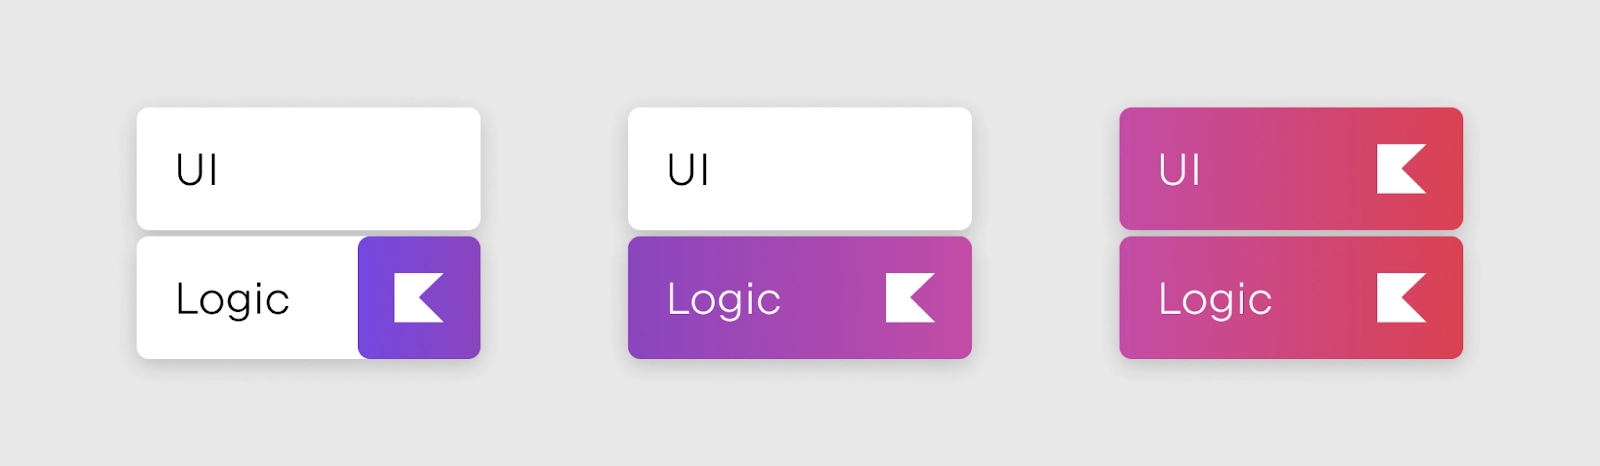
\includegraphics[width=150mm, keepaspectratio]{figures/KMP-types.png}
    \caption{A KMP fejlesztés változatai. \cite{KotlinMultiplatformStable}}
    \label{fig:KMPTypes}
\end{figure}

Semmi sem teljesen tökéletes így előfordulaht, hogy az egyik platformna máshogy, nem lehet vagy nem érdemes valamit megvalósítani, mint például egy asztali alaklmazáson egy fotó elkészítését az én példámban.
Ilyenkor jöhetnek szóba az expect és actual függvények. A közös kódan ilyenkor egy függvénytörzset definiálunk, csak itt lehet ebben az esetben alapértelmezett paramétereket beálítani, például egy Modifiert Composable függvény esetén.
A megvalósítás ilyenkor az alaklamzás specifikus kódban történik (androidMain, desktopMain, iOSMain). (\ref{lst:ExpectActual}.~kódrészlet)
Ehhez az actual functiont kell megvalósítani, és a platformtól függően ezek fognak meghívódni automatikusan, mivel a build során ezek lesznek behelyesítve az expect függvény helyére.
Már létezik actual és expect osztály is, én alkalmaztam is, de ez még kisérleti verzióban van.

\begin{lstlisting}[caption={Expect és actual használata}, label={lst:ExpectActual}, language=Kotlin]
//commonMain-ben lévű expect függvénytörzs, alapértelmezett paraméterrel.
@Composable
expect fun MainCameraScreen(examId: String = "0", navigateBack: () -> Unit)

//androidMain-ben lévő valós megvalósítás
@Composable
actual fun MainCameraScreen(examId: String, navigateBack: () -> Unit) {

    val cameraPermissionState: PermissionState = rememberPermissionState(android.Manifest.permission.CAMERA)

    MainCameraContent(
        hasPermission = cameraPermissionState.status.isGranted,
        examId = examId,
        onRequestPermission = cameraPermissionState::launchPermissionRequest,
        navigateBack = navigateBack
    )
}

//desktopMain-ben lévő placeholder megvalósítás, értesíti a felhasználót, hogy ez a funkció az eszközén nem támogatott
@Composable
actual fun MainCameraScreen(examId: String, navigateBack: () -> Unit) {
    Scaffold(
        topBar = {
            TopAppBarContent(stringResource(Res.string.camera), navigateBack)
                 },
        ){innerPadding ->
            UnsupportedFeatureScreen(modifier = Modifier.padding(innerPadding))
    }
}
\end{lstlisting}

\section{Gradle build rendszer}

A Compose Multiplatform projektek is a Gradle build rendszert használják, első sorban a függőségek megszerzésere és az alkalmazás létrehozására.
Egy átlagos fejlesztőnek mindösszesen annyi dolga van, hogy kigyűjti a használt függőségeket és a fejlesztőkörnyezet általában segít a megfelelő verziók megtalálásában.
Újbban a Kotlin DSL használata terjedt el.
"A DSL (Domain-Specific Language) egy programozási nyelv, amely egy meghatározott problémakör megoldására összpontosít. Az általános célú nyelvektől eltérően a DSL-ek, például az SQL és a regexek, csak egy szűk területre fókuszálnak, ami lehetővé teszi a problémák deklaratív módon való megoldását."\cite{KotlinDSL}
Ennek a segítségével egyszerűbben tudjuk megadni a Gradle függőségeket.(\ref{lst:KotlinDSL}.~kódrészlet)

\begin{lstlisting}[caption={Kotlin DSL}, label={lst:KotlinDSL}, language=Kotlin]
kotlin {    //Részlet a build.gradle fájlból
    androidTarget {
        compilerOptions {
            jvmTarget.set(JvmTarget.JVM_11)
        }
    }
    sourceSets {
        androidMain.dependencies {
            implementation(libs.androidx.activity.compose)
        }
    }
}
\end{lstlisting}

Ezen kívül a verziók egyszerűbb karbantartására használhatunk version catalog fájlt, ez a libs.version.toml.
A toml a "Tom's Obvious, Minimal Language" rövidítése, ezt első sorban egyszerűbb konfigurációs fájlok esetében használják, ha úgy tetszik egy "butább" yaml formátum.
Az szükséges részei a [versions] és a [libraries], illeve szükség lehet [plugins]-re is. (\ref{lst:toml}.~kódrészlet) Az itt felvett értékekre lehet hivatkozni a build.gradle fájl(ok)ban.

\begin{lstlisting}[caption={Version catalog}, label={lst:toml}, language=Kotlin]
#Részlet a libs.version.toml fájlból

[versions]
agp = "8.2.2"
android-compileSdk = "34"
android-minSdk = "24"
android-targetSdk = "34"
androidx-activityCompose = "1.9.2"
androidx-appcompat = "1.7.0"
androidx-constraintlayout = "2.1.4"
androidx-core-ktx = "1.13.1"

[libraries]
androidx-core = { module = "androidx.core:core", version.ref = "androidx-core-ktx" }
androidx-core-ktx-v1120 = { module = "androidx.core:core-ktx", version.ref = "coreKtx" }

[plugins]
androidApplication = { id = "com.android.application", version.ref = "agp" }
androidLibrary = { id = "com.android.library", version.ref = "agp" }
\end{lstlisting}


\section{Fejlesztőkörnyeztek}

Fejlesztőkörnyezetnek a JetBrains egyik eszközét választottam, a Fleet-et.
Kifejezetten Multiplatform fejlesztéshez készítettek, szinte az összes nyelvet támogata ami ebben a témában szóba jöhet, és minden funkcióval rendelkezik amivel a natív fejlesztésre készült IDE-ik is.
Többek között kódkiegészítéssel és kód kiemeléssel is, így nem kell IDE-t váltani, ha más nyelven kell éppen dolgozni.
"Amikor az Smart Mode engedélyezve van, a Fleet nyelvspecifikus funkciókat kínál, mint például a kódkiegészítés, navigáció, hibakeresés és refaktorálás. Ha ez a mód le van tiltva, a Fleet egyszerű szövegszerkesztőként működik; gyorsan meg lehet nyitni fájlokat és módosításokat végezni, de a fejlettebb funkciók nélkül. A háttérben a Fleet kiválasztja a kód feldolgozásához szükséges háttérmotort. Intelligens módban például a Kotlin feldolgozási motorja az IntelliJ IDEA-hoz használt motor, így ismerős funkciók maradnak elérhetők." \cite{Fleet}
Egy másik hasznos funkció, hogy egy helyről lehet minden platformra buildelni az alkalamzást (\refstruc{fig:RunConfigs}) így nem kell egy külön Android Studiot és egy Xcodeot is megynitni, ha szeretnéd tesztelni az alaklamzást az adott eszközön.

A fő fejlesztőkörnyezeten kívül amíg csak az Android applikációt fejleszettem az Android Studiot használtam.
A REST API megírásához és karbantarásához szintén a JetBrains termékét az IntelliJ IDEA Ultimate-et használtam, ami kifejezetten Java és Kotlin projekezhez készült.
Kisebb mértékben a fejlesztéshez és nagyobb mértékben a dokumentációhoz és a szakdolgozat megírásához A Visual Studio Code-ot használtam, mivel sok hasznos bővítménnyel rendelkezik például \LaTeX és PlantUML használatához.


\begin{figure}[!ht]
    \centering
    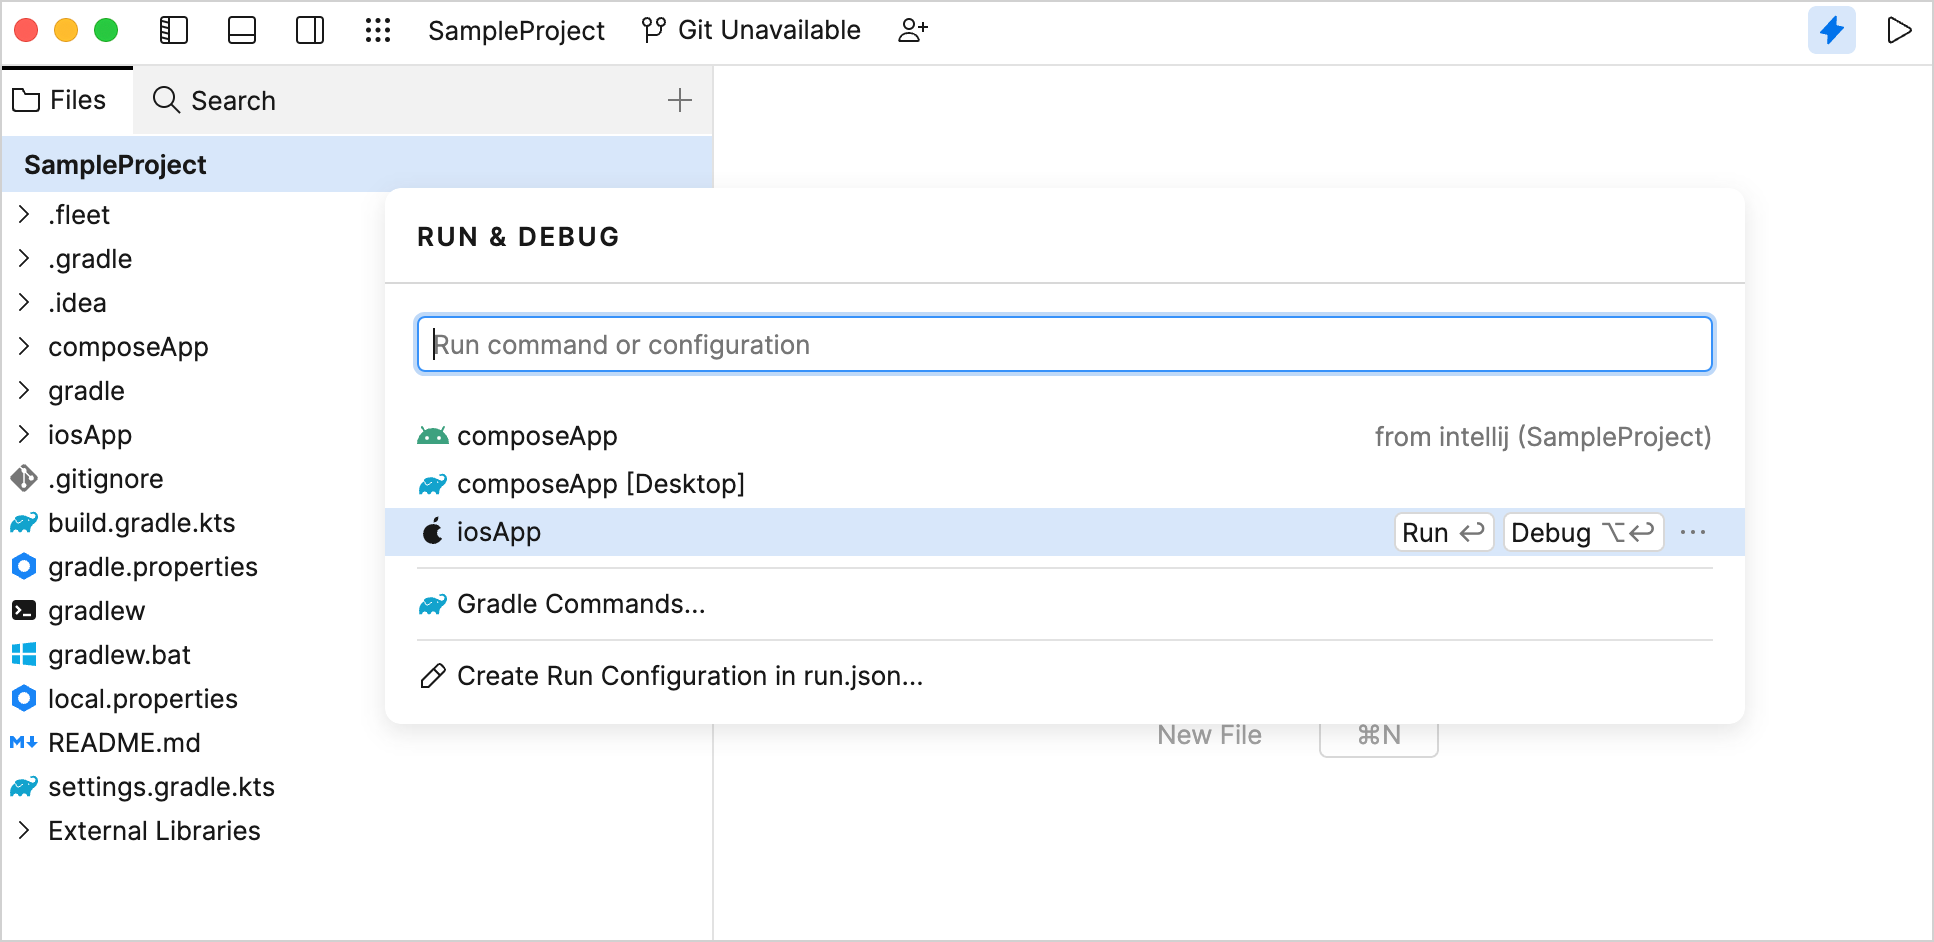
\includegraphics[width=150mm, keepaspectratio]{figures/fleet-run-configurations.png}
    \caption{A különböző eszközökre egy helyen lehet buildelni és futtani az alkalmazást. \cite{Fleet}}
    \label{fig:RunConfigs}
\end{figure}




\section{REST API, Postman és adatbázis}

\section{Dokumentáció: \LaTeX, PlantUML}


\section{Kipróbált, de végül nem használt egyéb érdekes megoldások}